
%(BEGIN_QUESTION)
% Copyright 2007, Tony R. Kuphaldt, released under the Creative Commons Attribution License (v 1.0)
% This means you may do almost anything with this work of mine, so long as you give me proper credit

Tegn bare integralresponsen til en regulator med {\it proporsjonal + integralvirkning}, med proporsjonalbånd 50\% og integralkonstant 4 minutter per repetisjon, for følgende inngangsbetingelser. Anta at regulatoren er {\it reversvirkende}:

$$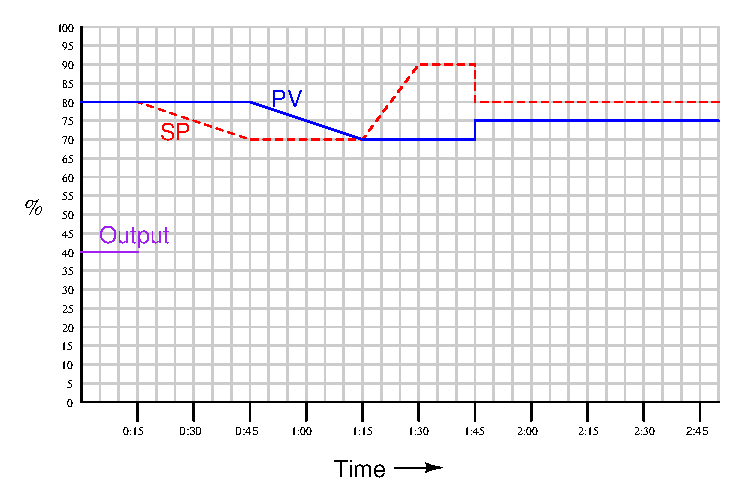
\includegraphics[width=15.5cm]{i01607x01.eps}$$

Tidsskalaen i diagrammet er minutter:sekunder, og PI-algoritmen er som følger:

$$m = K_p \left( e + {1 \over \tau_i} \int e \> dt \right) + b$$

\noindent
Der,

$m$ = regulatorutgang (manipulert variabel)

$K_p$ = forsterkning

$e$ = avvikssignal (SP$-$PV)

$\tau_i$ = integraltidskonstant

$b$ = bias

\vskip 10pt

\underbar{file i01607}
%(END_QUESTION)





%(BEGIN_ANSWER)

$$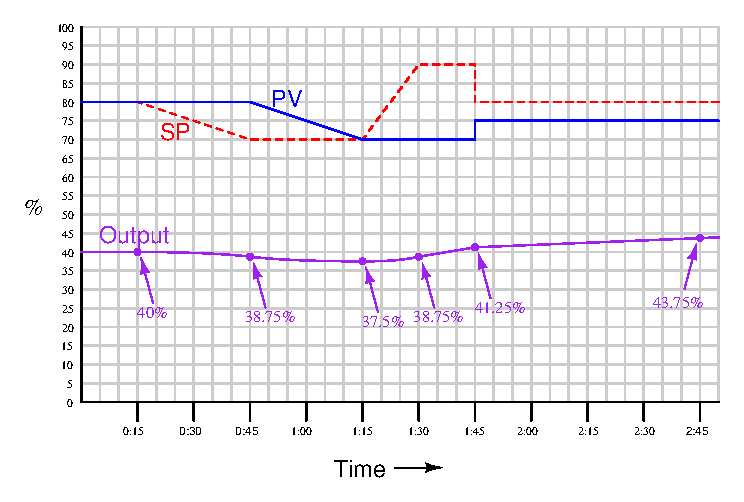
\includegraphics[width=15.5cm]{i01607x02.eps}$$

Først konverterer vi de oppgitte tune-konstantene til direkte visende enheter (forsterkning i stedet for P.B., og rep/min i stedet for min/rep):
 
\vskip 10pt

Proporsjonalbånd = 50\% ; Forsterkning = 2
 
\vskip 10pt

4 minutter per repetisjon = 0.25 repetisjoner per minutt
 
\vskip 10pt
 
\noindent
Deretter beregner vi akkumulert areal under hver avviksperiode:
 
\vskip 10pt
 
Integralvirkning = $K_p {1\over \tau_i} \int e \> dt$
 
\vskip 10pt

Integralvirkning = (forsterkning)(repetisjoner/min)(avvik-tid-produkt)
 
\vskip 10pt

Integralvirkning = (2)(0.25/min)(2.5\%-min)
 
\vskip 10pt

Integralvirkning = 1.25\%
 
\vskip 10pt

\noindent
{\it Utgangen går fra 40\% til 38.75\%}

$$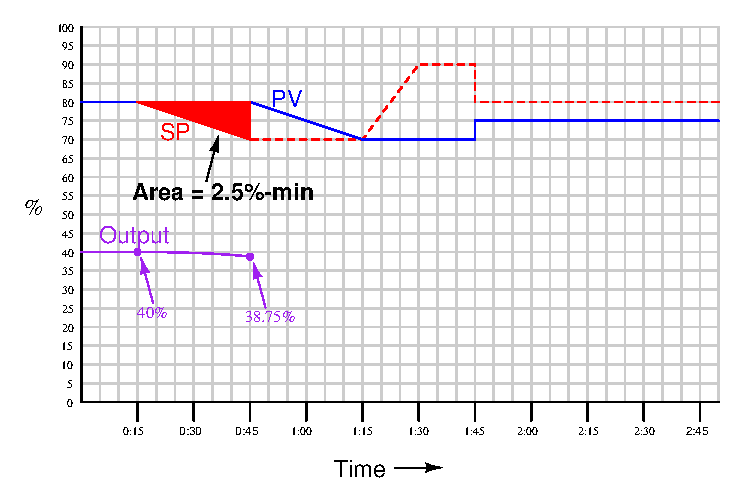
\includegraphics[width=15.5cm]{i01607x03.eps}$$

\filbreak 

Integralvirkning = $K_p {1\over \tau_i} \int e \> dt$
 
\vskip 10pt

Integralvirkning = (forsterkning)(repetisjoner/min)(avvik-tid-produkt)
 
\vskip 10pt

Integralvirkning = (2)(0.25/min)(2.5\%-min)
 
\vskip 10pt

Integralvirkning = 1.25\%
 
\vskip 10pt
 
\noindent
{\it Utgangen går fra 38.75\% til 37.5\%}
 
$$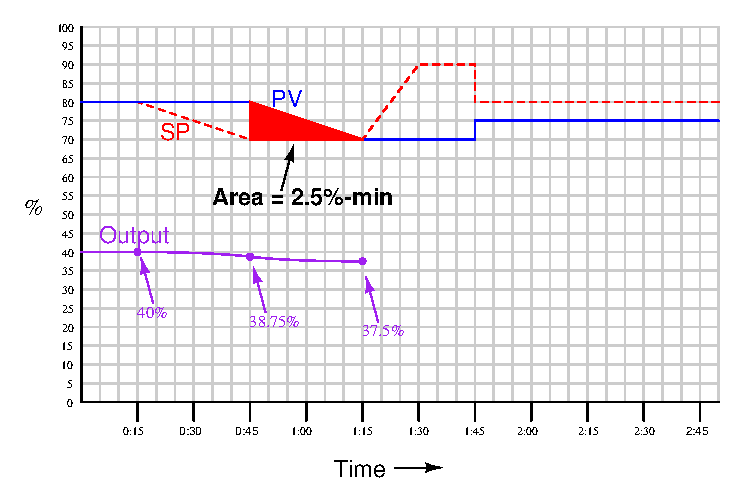
\includegraphics[width=15.5cm]{i01607x04.eps}$$

\filbreak 

Integralvirkning = $K_p {1\over \tau_i} \int e \> dt$
 
\vskip 10pt

Integralvirkning = (forsterkning)(repetisjoner/min)(avvik-tid-produkt)
 
\vskip 10pt

Integralvirkning = (2)(0.25/min)(2.5\%-min)
 
\vskip 10pt

Integralvirkning = 1.25\%
 
\vskip 10pt
 
\noindent
{\it Utgangen går fra 37.5\% til 38.75\%}
 
$$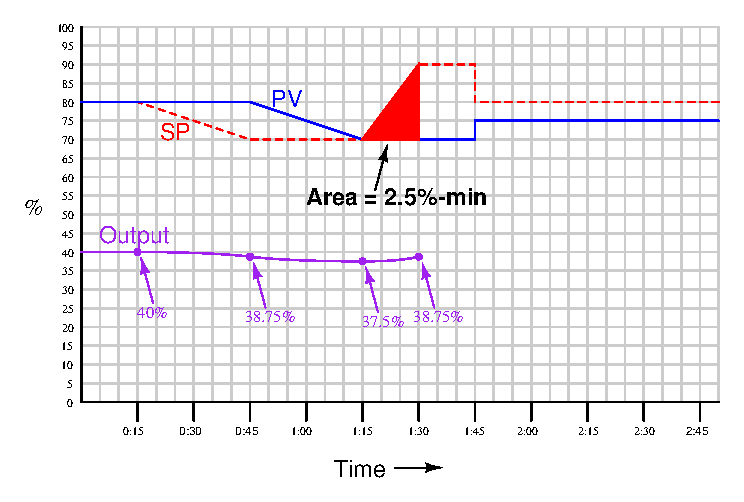
\includegraphics[width=15.5cm]{i01607x05.eps}$$

\filbreak 

Integralvirkning = $K_p {1\over \tau_i} \int e \> dt$
 
\vskip 10pt

Integralvirkning = (forsterkning)(repetisjoner/min)(avvik-tid-produkt)
 
\vskip 10pt

Integralvirkning = (2)(0.25/min)(5\%-min)
 
\vskip 10pt

Integralvirkning = 2.5\%
 
\vskip 10pt
 
\noindent
{\it Utgangen går fra 38.75\% til 41.25\%}
 
$$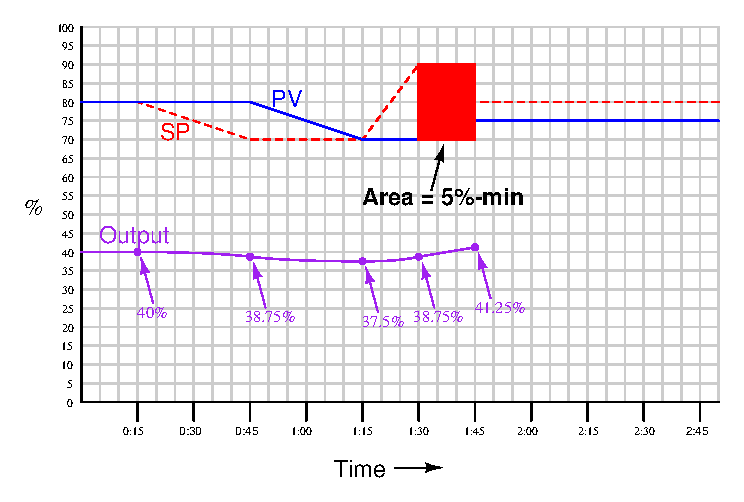
\includegraphics[width=15.5cm]{i01607x06.eps}$$
 
\filbreak 

Integralvirkning = $K_p {1\over \tau_i} \int e \> dt$
 
\vskip 10pt

Integralvirkning = (forsterkning)(repetisjoner/min)(avvik-tid-produkt)
 
\vskip 10pt

Integralvirkning = (2)(0.25/min)(5\%-min)
 
\vskip 10pt

Integralvirkning = 2.5\%
 
\vskip 10pt

\noindent
{\it Utgangen går fra 41.25\% til 43.75\%}
 
$$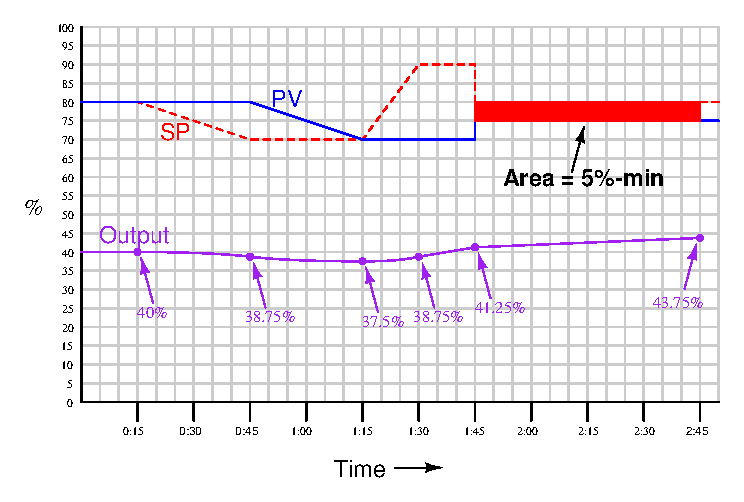
\includegraphics[width=15.5cm]{i01607x07.eps}$$

%(END_ANSWER)





%(BEGIN_NOTES)


%INDEX% Control, proportional + integral: graphing controller response

%(END_NOTES)
